%%%%%%%%%%%%%%%%%%%%%%%%%%%%%%%%%%%%%%%%%
% Lachaise Assignment
% LaTeX Template
% Version 1.0 (26/6/2018)
%
% This template originates from:
% http://www.LaTeXTemplates.com
%
% Authors:
% Marion Lachaise & François Févotte
% Vel (vel@LaTeXTemplates.com)
%
% License:
% CC BY-NC-SA 3.0 (http://creativecommons.org/licenses/by-nc-sa/3.0/)
% 
%%%%%%%%%%%%%%%%%%%%%%%%%%%%%%%%%%%%%%%%%

%----------------------------------------------------------------------------------------
%	PACKAGES AND OTHER DOCUMENT CONFIGURATIONS
%----------------------------------------------------------------------------------------
\documentclass{article}

\input{structure.tex} % Include the file specifying the document structure and custom commands

\usepackage{amsmath}
\usepackage{amsthm}
\usepackage{amsfonts}
\usepackage{amssymb}

\usepackage{listings}

\usepackage{color}

\definecolor{green}{RGB}{28,172,0} % color values Red, Green, Blue

\definecolor{lilas}{RGB}{170,55,241}

\lstset{language=Matlab,%
    %basicstyle=\color{red},
    breaklines=true,%
    morekeywords={matlab2tikz},
    keywordstyle=\color{blue},%
    morekeywords=[2]{1}, keywordstyle=[2]{\color{black}},
    identifierstyle=\color{black},%
    stringstyle=\color{lilas},
    commentstyle=\color{green},%
    showstringspaces=false,%without this there will be a symbol in the places where there is a space
    numbers=left,%
    numberstyle={\tiny \color{black}},% size of the numbers
    numbersep=9pt, % this defines how far the numbers are from the text
    emph=[1]{for,end,break},emphstyle=[1]\color{red}, %some words to emphasise
    %emph=[2]{word1,word2}, emphstyle=[2]{style},    
}

\usepackage{graphicx}
\usepackage[format=plain,
            labelfont={bf,it},
            textfont=it]{caption}
%----------------------------------------------------------------------------------------
%	ASSIGNMENT INFORMATION
%----------------------------------------------------------------------------------------

\title{Accuracy of Numerical Methods to Diffusion Equations} % Title of the assignment

\author{Xinyi Li\\ \texttt{xinyi.li4@uq.net.au}} % Author name and email address

\date{The University of Queensland --- \today} % University, school and/or department name(s) and a date

%----------------------------------------------------------------------------------------

\begin{document}

\maketitle % Print the title

%----------------------------------------------------------------------------------------
%	INTRODUCTION
%----------------------------------------------------------------------------------------

\section*{Abstract} % Unnumbered section

Deriving from a series of random walks, the diffusion equation is one of the most important partial differential equation. This equation allows us to model and predict the distribution of particles after some time over a region and with careful tweaking models of many instances can be created to a high. This project will model different cases of the equation and provide an analysis of the stability and accuracy of the cases.

\section{Introduction} % Numbered section

Taking the diffusion equation, we can adjust the terms and the conditions of the model to provide a more real and accurate prediction of a system. With some controlled adjustment models of heat distribution, the spread of cells or species and even signals can be generated. To obtain an accurate model, however, additional terms are added to the standard diffusion equation which could make it more difficult or impossible to solve. Thus, numerical methods such as the finite difference Scheme or the finite element method will be used to approximate solutions to such equations.
\\
\\
In this project, we will test the accuracy and stability of numerical solutions to different forms of the diffusion equations. In each case, we will attempt to find an analytical solution if available then approximate and compare the solutions to a numerical approximation. Additionally, the stability and speed of the numerical solution will be considered to predict whether if the model is feasible on a larger scale.
%------------------------------------------------

\section{Models \& Methods}

Four models will be considered, the system of the models will be derived from the standard diffusion equation with adjustments such as adding an extra term or changing the boundary conditions. The new systems will cover types including homogeneous/non-homogeneous systems, linear/non-linear systems with Dirichlet/Neumann boundary conditions.
\\
\\
We will consider the cases below, and additionally perform error and runtime comparisons of the methods.
\begin{itemize}
\item Case A, Homogeneous Dirichlet zero flux boundary condition.
\item Case B, Homogeneous Dirichlet boundary condition.
\item Case C, Non-Homogeneous Dirichlet boundary condition.
\item Case D, Nonlinear model.
\end{itemize}

For each model, an analytical solution will be first calculated if possible. Numerically, we will approximate the system using the finite difference method and MATLAB's built-in PDE solver, 'pdepe'. The models are greatly simplified where the main dynamics are the influx or outflux of particles. This allows analytical solutions to be derived and reduces the possibility of unknown systems such as a stiff system causing problems for our numerical methods.
\\
\\
Standard conventions of solving diffusion equations will be applied to derive the analytical result. For the standard case, we will apply separation of variables to the equation and derive a Fourier series. In the case of B, we will use the error function and the delta function to derive a formula for the diffusion equation on an infinite domain. Finally, in the last case, we will attempt to calculate the equilibrium solution and eliminate the time dependence and compare the numerical methods to the equilibrium solution.
	
%------------------------------------------------

\section{Theory}

\subsection{Homogeneous Boundary Condition with Separation of Variables}

For the systems where the boundary condition is homogeneous, we can derive a series of linear solutions satisfying the boundary condition. Then using the superposition principle we can construct a general solution to the PDE which will be the basis of our analytical solution to the diffusion equation. To begin, we will apply the separation of variables,
\[
	\begin{split}
		\frac{\partial u}{\partial t} &= k\frac{\partial^2 u}{\partial x^2} \\
		\text{Let} \ u(x, t) &= g(t)h(x) \\
		\therefore \ \frac{\partial g(t)h(x)}{\partial t} &= k\frac{\partial^2 g(t)h(x)}{\partial x^2}
	\end{split}
\]
Rearrange and we get,
\[
	\begin{split}
		\frac{1}{kg(t)} \cdot \frac{\partial g(t)}{\partial t} &= \frac{1}{h(x)}\cdot \frac{\partial^2 h(x)}{\partial x^2} = -\lambda \ \text{\small for} \ \lambda > 0
	\end{split}
\]
\begin{equation}
\label{eq:a}
\frac{1}{kg(t)} \cdot \frac{\partial g(t)}{\partial t} = -\lambda
\end{equation}
\begin{equation}
\label{eq:b}
\frac{1}{h(x)}\cdot \frac{\partial^2 h(x)}{\partial x^2} = -\lambda
\end{equation}
Equation (1) and (2) are now ODEs, we can solve them separately.
\\
Equation (1),
\[
	\begin{split}
		\frac{1}{kg(t)} \cdot \frac{\partial g(t)}{\partial t} &= -\lambda \\
		\frac{1}{g(t)}dg &= -k\lambda \ dt \\
		\int \frac{1}{g(t)}dg &= \int -k\lambda \ dt \\
		\ln|g(t)| &= -kt\lambda + C \\
		\therefore \ g(t) &= Ae^{-kt\lambda}
	\end{split}
\]
Equation (2),
\[
	\begin{split}
		h(x) &= A\sin{(\sqrt{\lambda}x)} + B\cos{(\sqrt{\lambda}x)} \\
	\end{split}
\]
Apply the left end boundary condition,
\[
	\begin{split}
		u(0, t) &= 0 \\
		\implies h(0) &= A\sin{(\sqrt{\lambda}0)} + B\cos{(\sqrt{\lambda}0)} = 0 \\
		\implies B &= 0 \\
	\end{split}
\]
Apply the right end boundary condition,
\[
	\begin{split}
		u(L, t) &= 0 \\
		\implies h(L) &= A\sin{(\sqrt{\lambda}L)} = 0 \\
		\therefore \ \sqrt{\lambda}L &= n\pi \\
		\lambda &= \left(\frac{n\pi}{L}\right)^2 \\
		\therefore \ h(x) &= A\sin{\left(\frac{n\pi}{L}x\right)} \\
		\therefore \ g(t) &= Ae^{-kt\left(\frac{n\pi}{L}\right)^2}
	\end{split}
\]
This gives us the general solution,
\begin{equation}
\label{eq:c}
u_n(x,t)=A_n\sin{\left(\frac{n\pi}{L}x\right)}e^{-kt\left(\frac{n\pi}{L}\right)^2} \ n=1,2,...
\end{equation}
\subsection{Fourier Series}
Derived from above, equation (3) satisfies the boundary condition for any $n$. By the superposition principle, we can express the solution to the diffusion equation with homogeneous boundary condition as a series. Therefore, 
\begin{equation}
\label{eq:d}
	u(x,t) = \sum^{\infty}_{n=0} A_n\sin{\left(\frac{n\pi}{L}x\right)}e^{-kt\left(\frac{n\pi}{L}\right)^2}
\end{equation}
Now consider the initial condition,
\[
	\begin{split}
		u(x,0) &= \sum^{\infty}_{n=0} A_n\sin{\left(\frac{n\pi}{L}x\right)}
	\end{split}
\]
Let,
\[
	\begin{split}
		f(x) &= \sum^{\infty}_{n=0} A_n\sin{\left(\frac{n\pi}{L}x\right)}
	\end{split}
\]
Deriving a formula for the initial condition,
\[
	\begin{split}
		f(x) &= \sum^{\infty}_{n=0} A_n\sin{\left(\frac{n\pi}{L}x\right)} \\
		f(x)\sin{\left(\frac{m\pi}{L}x\right)} &= \sum^{\infty}_{n=0} A_n\sin{\left(\frac{n\pi}{L}x\right)}\sin{\left(\frac{m\pi}{L}x\right)} \\
		\int_{-L}^{L} f(x)\sin{\left(\frac{m\pi}{L}x\right)} \ dx & = \int_{-L}^{L} A_n\sin{\left(\frac{n\pi}{L}x\right)}\sin{\left(\frac{m\pi}{L}x\right)} \ dx
	\end{split}
\]
The above integral will be non-zero if $n=m$, therefore we can rewrite it as
\[
	\begin{split}
		A_nL &= \int_{-L}^{L} f(x)\sin{\left(\frac{n\pi}{L}x\right)} \ dx  \\
		A_n &= \frac{1}{L} \int_{-L}^{L} f(x)\sin{\left(\frac{n\pi}{L}x\right)} \ dx\\
		&=\frac{2}{L} \int_{0}^{L} f(x)\sin{\left(\frac{n\pi}{L}x\right)} \ dx
	\end{split}
\]
Therefore the truncated series is
\[
	u(x,t) = \sum^{\infty}_{n=0} A_n\sin{\left(\frac{n\pi}{L}x\right)}e^{-kt\left(\frac{n\pi}{L}\right)^2}
\]
where
\[
	A_n = \frac{2}{L} \int_{0}^{L} f(x)\sin{\left(\frac{n\pi}{L}x\right)} \ dx
\]

\subsection{Non-Homogeneous Boundary Values}
The above truncated series will only satisfy homogeneous boundary conditions. Here we will modify the steps slightly and derive a new series for non homogeneous boundary conditions.

Finding a solution of the form,
\[
	\begin{split}
		u(x, t) = u_s(x) + v(x, t)
	\end{split}
\]
Where $u_s(x)$ is the steady state solution of the system, i.e.
\[
	\begin{split}
		\lim_{t\rightarrow\infty} u(x, t) = u_s(x)
	\end{split}
\]
Should the steady state solution satisfy the boundary values, then we can generate a solution to the overall boundary value problem. Let,
\[1
	\begin{split}
		u_s(0) = A \\
		u_s(L) = B \\
		u_s(x) = C_1x + C_2
	\end{split}
\]
\[
	\begin{split}
		u_s(0) = C_2 = A \\
		u_s(L) = C_1L + A \\
		C_1 = \frac{u_s(L) - A}{L} \\
		\therefore u_s(x) = \frac{B - A}{L}x + A
	\end{split}
\]
Where,
\[
	\begin{split}
		v(x, t) &= \sum^{\infty}_{n = 1}C_n\sin{\left(\frac{\pi nx}{L}\right)}e^{-D\left(\frac{n\pi}{L}\right)^2t} \\
		C_n &= \frac{2}{L}\int^L_0 (f(x) - h(x))\sin{\left(\frac{n\pi x}{L}\right)} \ dx
	\end{split}
\]
The final equation is
\[
	\begin{split}
		u(x, t) = A + \frac{B - A}{L}x + \sum^{\infty}_{n=1}C_n\sin{\left(\frac{\pi nx}{L}\right)}e^{-D\left(\frac{n\pi}{L}\right)^2t}
	\end{split}
\]
\subsection{Non-Linear Systems}
Consider the system, with Homogeneous Dirichlet Boundary Condition
\[
	\begin{split}
		\frac{\partial u}{\partial t} &= \frac{\partial^2 u}{\partial x^2} + S(x)
	\end{split}
\]
Where $S(x)$ is some constant particle distribution area at $x$.
Although we cannot generate a Fourier series solution for this system, we can consider the steady state solution similar to the system specified in section 3.3
\[
	\begin{split}
		\lim_{t\rightarrow\infty}u(x,t)&=u_s(x)
	\end{split}
\]
Suppose the area exists between $a$ and $b$ i.e.
\[ 
	S(x) = \begin{cases} 
      0 & -L \leq x < A \\
      1 & A\leq x\leq B \\
      0 & B < x \leq L
   \end{cases}
\]
Then we can solve the equation on the separate domains [-L,A), (A,B) and (B,L].

\noindent Case 1, $[-L,A)$ with boundary condition $u(-L) = 0$
\[
	\begin{split}
		D\frac{\partial^2 u}{\partial x^2} &= -L \\
		\iint D\frac{\partial^2 u}{\partial x^2} &= \iint 0 \ dx \\
		u(x) &= ax + b \\
		u(-L) &= -aA + b = 0\\
		\therefore \ b &= aA
	\end{split}
\]
Case 2, $[A,B]$.
\[
	\begin{split}
		D\frac{\partial^2 u}{\partial x^2} &= -1 \\
		\iint D\frac{\partial^2 u}{\partial x^2} &= \iint -1 \ dx \\
		u(x) &= \frac{-x^2}{2} + cx + d
	\end{split}
\]
Assume that the temperature is evenly distributed we have,
\[
	\begin{split}
		u(A) &= u(B) \\
		\frac{-A^2}{2} + Ac + d &= \frac{-B^2}{2} + Bc + d \\
		\frac{-A^2}{2} + Ac &= \frac{-B^2}{2} + Bc \\
		-A^2 + 2Ac &= -B^2 + 2Bc \\
		2Ac - 2Bc &= A^2 - B^2 \\
		\therefore \ c = \frac{A^2 - B^2}{2A - 2B}
	\end{split}
\]
Case 3, $(B,L]$ with boundary condition $u(L) = 0$
\[
	\begin{split}
		0 &= D\frac{\partial^2 u}{\partial x^2} \\
		\iint D\frac{\partial^2 u}{\partial x^2} &= \iint 0 \ dx \\
		u(x) &= ex + f \\
		u(L) &= eB + f = 0\\
		\therefore \ f &= -eB
	\end{split}
\]
The final steady state solution of the system can be evaluated as
\[ u_s(x) = \begin{cases} 
      ax + b & -L \leq x < A \\
      \frac{-x^2}{2} + cx + d & A \leq x\leq B \\
      ex + f & B < x \leq L
   \end{cases}
\]
\newpage
%------------------------------------------------
\section{Algorithms}
\subsection{Overview}
As mentioned before, the main numerical methods we will apply is the pdepe() function and the Finite Difference Scheme. Since pdepe() is already a MATLAB built in function, the only additional algorithm we required is the Finite Difference Scheme.
\\
\\
pdepe() utilizes the method of lines and the finite element method to approximate the spacial values. Then solutions at time $t$ is solved with the ODE solver ode15s. We can expect pdepe to work in most cases since the methods are of low order, thus it reduces problematic systems such as stiff systems that may cause long run times or unstable solutions. As a consequence, the accuracy of the solution may vary depending on the system and the step size we have chosen, especially with the truncation error generated by the Fourier series.
\\
\\
The Finite Difference Scheme on the other hand, is a extension of the 1D Finite Difference Scheme used to approximate ODE's, but rather than approximating one point, we will approximate a set of points at time $t+1$ using spatial values at the current time. For Dirichlet boundary conditions, the boundaries are a vector of values equal to what is specified by the boundary condition. Neumann boundary conditions however will require some tweaking and will require the boundary values to be generated along with the middle points. 

\subsection{Implementation}
Below, We will implement two explicit Finite Difference Scheme method, one for Dirichlet boundary conditions and the other for Neumann boundary conditions.
\\
\\
Approximating the value at $t+1$ and $x+1$with a small step, we have
\[
	u(x,t)=u(x+\triangle x, t+\triangle t)=u^l_k
\]
Taking the forward difference at time $t$ and the central difference at a set of points $x_k$ the approximation can be expressed as
\[
	\frac{u^{l+1}_k-u^l_k}{\triangle t}=D\left(\frac{u_{k+1}^l-u_k^l}{(\triangle x)^2}-\frac{u_k^l-u_{k-1}^l}{(\triangle x)^2}\right)
\]
Rearrange for the required result of,
\[
	u^{l+1}_k=u^l_k+D\frac{\triangle t}{(\triangle x)^2}\left(u^l_{k+1}-2u^l_k+u^l_{k-1}\right)
\]
For Dirichlet boundary condition set,
\[
	\begin{split}
		u(a,t) &= A \\
		u(b,t) &= B \\
	\end{split}
\]
For Neumann boundary condition, we will approximate the boundary values using the central difference method,
\[
	\begin{split}
		\frac{u^l_1-u^l_0}{\triangle x} &= A \\
		\frac{u^l_k-u^l_{k-1}}{\triangle x} &= B \\
	\end{split}
\]
FDM.m Finite Difference Method - Dirichlet Boundary Conditions.
\begin{lstlisting}[language=MATLAB]
% Finite Difference Method with Dirichlet Boundary Conditions.
% Inputs:
% D - Diffusion Coefficient
% dx - Spatial step size
% dt - time step size
% xbound - Boundaries for x
% tbound - Boundaries for t
% bc - Boundary values at the end points
% ic - Initial condition
% Outputs:
% U - Solution to the diffusion equation.
function U=FDM(D,dx,dt,xbound,tbound,bc,ic)
    x_vec=xbound(1):dx:xbound(2);
    t_vec=tbound(1):dt:tbound(2);
    U=zeros(length(x_vec),length(t_vec));
    U(1,:)=bc(1);
    U(end,:)=bc(2);
    U(:,1)=ic(xbound(1):dx:xbound(2));
    for t=1:length(t_vec)-1
        for x=2:length(x_vec)-1
            U(x,t+1)=U(x,t)+(D*dt/dx^2)*(U(x+1,t)-2*U(x,t)+U(x-1,t));
       end
    end
end
\end{lstlisting}
FDMNeumann.m Finite Difference Method - Neumann Boundary Conditions.
\begin{lstlisting}[language=MATLAB]
% Finite Difference Method with Neumann Boundary Conditions.
% Inputs:
% D - Diffusion Coefficient
% dx - Spatial step size
% dt - time step size
% xbound - Boundaries for x
% tbound - Boundaries for t
% bc - Boundary values at the end points
% ic - Initial condition
% Outputs:
% U - Solution to the diffusion equation.
function U=FDMNeumann(D,dx,dt,xbound,tbound,bc,ic)
    x_vec=xbound(1):dx:xbound(2);
    t_vec=tbound(1):dt:tbound(2);
    U=zeros(length(x_vec),length(t_vec));
    U(1,:)=bc(1);
    U(end,:)=bc(2);
    U(:,1)=ic(xbound(1):dx:xbound(2));
    for t=1:length(t_vec)-1
        U(1,t+1)=U(1,t)+(D*dt/dx^2)*(U(2,t)-2*U(1,t)+bc(1));
        for x=2:length(x_vec)-1
            U(x,t+1)=U(x,t)+(D*dt/dx^2)*(U(x+1,t)-2*U(x,t)+U(x-1,t));
        end
        U(x+1,t+1)=U(x+1,t)+(D*dt/dx^2)*(bc(2)-2*U(x+1,t)+U(x,t));
        bc(1)=U(2,t+1);
        bc(2)=U(x,t+1);
    end
end
\end{lstlisting}
FDMInitial.m Finite Difference Method - Dirichlet Boundary Conditions. Allows a domain of diffusing particles to be specified.
\begin{lstlisting}[language=MATLAB]
% Finite Difference Method with Dirichlet Boundary Conditions
% Allows a domain of constant diffusing particles to be specified.
% Inputs:
% D - Diffusion Coefficient
% dx - Spatial step size
% dt - time step size
% xbound - Boundaries for x
% tbound - Boundaries for t
% bc - Boundary values at the end points
% ic - Initial condition
% fd - Field bounds, where the constant input area is defined.
% Outputs:
% U - Solution to the diffusion equation.
function U=FDMInitial(D,dx,dt,xbound,tbound,bc,ic,fd)
    x_vec=xbound(1):dx:xbound(2);
    t_vec=tbound(1):dt:tbound(2);
    U=zeros(length(x_vec),length(t_vec));
    U(1,:)=bc(1);
    U(end,:)=bc(2);
    U(:,1)=ic;
    for t=1:length(t_vec)-1
        for x=2:length(x_vec)-1
            xk=x*dx;
            if (xk < 0.2 && xk > 0.1) || (xk < 0.9 && xk > 0.8)
                U(x,t+1)=U(x,t)+(D*dt/dx^2)*(U(x+1,t)-2*U(x,t)+U(x-1,t))+1*dt;
            else
                U(x,t+1)=U(x,t)+(D*dt/dx^2)*(U(x+1,t)-2*U(x,t)+U(x-1,t));
            end
       end
    end
end
\end{lstlisting}
\subsection{Stability}
It is necessary to consider the stability of the solution iterated at each point and ensure that the output result are within some tolerance. In order for the Finite Difference Scheme to converge to a adequate solution, it should satisfy a condition when the step sizes are chosen.
\\
\\
Suppose we add some errors to the system.
\[
	u^{l+1}_k + \delta^{l}_{k} = u^l_k+D\frac{\triangle t}{(\triangle x)^2}\left(u^l_{k+1}-2u^l_k+u^l_{k-1}\right) + \delta^{l+1}_{k}
\]
Where
\[
	\delta^{l}_{k} = \sum_{n=0}^{\infty} A_ne^{i\frac{n\pi}{2L}(k\triangle x)}
\]
We want the error to not be amplified/growing. Define the amplification factor,
\[
	A_f = \frac{\delta^{l+1}_{k}}{\delta^{l}_{k}}
\]
Keeping this factor below or equal to 1 allows the error to stay steady or decrease, i.e
\[
	A_f \leq 1
\]
Substitute $\delta$ in to the original system we have,
\[
	\begin{split}
		\delta^{l+1}_k &= \delta^l_k+D\frac{\triangle t}{(\triangle x)^2}\left(\delta^l_{k+1}-2\delta^l_k+\delta^l_{k-1}\right) \\
		&= A_ne^{i\frac{n\pi}{2L}(k\triangle x)}+A_n D\frac{\triangle t}{(\triangle x)^2}\left(e^{i\frac{n\pi}{2L}((k+1)\triangle x)}-2e^{i\frac{n\pi}{2L}(k\triangle x)}+e^{i\frac{n\pi}{2L}((k-1)\triangle x)}\right) \\
		&= A_ne^{i\frac{n\pi}{2L}(k\triangle x)}\left(1+D\frac{\triangle t}{(\triangle x)^2}\left(e^{i\frac{n\pi}{2L}\triangle x}-2+e^{-i\frac{n\pi}{2L}\triangle x}\right)\right) \\
		&= \delta^l_k\left(1+2D\frac{\triangle t}{(\triangle x)^2}\left(\cos{\left(\frac{n\pi}{2L}k\triangle x\right)}-1\right)\right) \\
		&= \delta^l_k\left(1+4D\frac{\triangle t}{(\triangle x)^2}\sin^2{\left(\frac{n\pi}{4L}\triangle x\right)}\right)
	\end{split}
\]
Now express the amplification factor as
\[
	\begin{split}
		A_f = \frac{\delta^{l+1}_{k}}{\delta^{l}_{k}} = 2D\frac{\triangle t}{(\triangle x)^2}\sin^2{\left(\frac{n\pi}{4L}\triangle x\right)}
	\end{split}
\]
Since
\[
	\begin{split}
		\sin^2{\left(\frac{n\pi}{4L}\triangle x\right)} < 1 \ \ \ \ \forall n,\triangle x,L \in \mathbb{R}
	\end{split}
\]
Then this term will not contribute to the amplification of the error and can be removed.
\[
	\begin{split}
		A_f &= 2D\frac{\triangle t}{(\triangle x)^2} \leq 1 \\
		\therefore \ \triangle t &\leq \frac{(\triangle x)^2}{2D}
	\end{split}
\]
Finally, for the Finite Difference Scheme to converge to an adequate solution, the above condition must be satisfied when step size are chosen. We will ensure our scripts satisfy this condition.
\newpage
\subsection{Utility}
seriesSum.m for summing Fourier Serires defined in the function handler 'series' up to the N'th term
\begin{lstlisting}[language=MATLAB]
% Function to sum a series up to n.
% Inputs:
% series - The function handler to the series function.
% x - The x values
% t - The t values
% n - The iteration to sum the series.
% Output:
% S - The total sum of the series.
function S=seriesSum(series,x,t,n)
S=0;
i=1;
    while (i<n+1)
        S=S+series(x,t,i);
        i=i+1;
    end
end
\end{lstlisting}
ErrorComparison.m Compares errors of both methods with respect to the Fourier Series.
\begin{lstlisting}[language=MATLAB]
% Comparison of Errors of pdepe() and FDM
function ErrorComparison
clear;
close all;

% Initial variables.
D=1; % Diffusion coefficient.
x_min=0; % Min domain
x_max=1; % Max domain
t_max=1; % Max time
xv=linspace(x_min,x_max,50); % Spatial vector 
dx=xv(2)-xv(1); % x step size
dt=0.5*(dx^2)/(2*D); % t stable step size
tv=0:dt:t_max; % Time vector

% Fourier series solution.
a0=0;
% Series for the domain [0,1]. Requires recalculation should domain change.
series=@(x,t,n)2*(-(pi*n*sin(pi*n)+2*cos(pi*n)-2)/(pi^3*n^3))*sin(n*pi*x)*exp(-(n*pi)^2*t);

% FDM Solution
ic=@(x)x.*(1-x);
fdmU=FDM(1,dx,dt,[x_min x_max],[0 t_max],[0 0],ic);
fdmU=fdmU';

% pdepe Solution
sol=pdepe(0,@pdex1pde,@pdex1ic,@pdex1bc,xv,tv);
% Extract the first solution component as u.
pdepeU=sol(:,:,1);

% Error Figures
figure
N=50;
hold on
for i=1:N
   loglog(xv,abs((seriesSum(series,xv,0,i))-fdmU(1,:)));
end
title('Comparison of FDM Error')
xlabel('Domain x')
ylabel('Error')
legend('Fourier Series Sum 1','Fourier Series Sum 2','Fourier Series Sum 3','Fourier Series Sum 4','Fourier Series Sum ...')
xlim([x_min x_max])

% Error Figures
figure
N=50;
hold on
for i=1:N
   loglog(xv,abs((seriesSum(series,xv,0,i))-pdepeU(2,:)));
end
title('Comparison of pdepe() Error')
xlabel('Domain x')
ylabel('Error')
legend('Fourier Series Sum 1','Fourier Series Sum 2','Fourier Series Sum 3','Fourier Series Sum 4','Fourier Series Sum ...')
xlim([x_min x_max])

% Pdepe function handlers
function [c,f,s]=pdex1pde(x,t,u,DuDx)
c=1;
f=DuDx;
s=0;

function u0=pdex1ic(x)
u0=x*(1-x);

function [pl,ql,pr,qr]=pdex1bc(xl,ul,xr,ur,t)
pl=0;
ql=ul;
pr=0;
qr=ur;
\end{lstlisting}
Runtime.m Compares runtimes of the methods used.
\begin{lstlisting}[language=MATLAB]
% Comparison of Runtimes of pdepe() and FDM
function Runtime
clear;
close all;

% Initial variables.
D=1; % Diffusion coefficient.
x_min=0; % Min domain
x_max=1; % Max domain
t_max=1; % Max time
xv=linspace(x_min,x_max,50); % Spatial vector 
dx=xv(2)-xv(1); % x step size
dt=0.5*(dx^2)/(2*D); % t stable step size
ic=@(x)x.*(1-x);

% Fourier series solution.
a0=0;
% Series for the domain [0,1]. Requires recalculation should domain change.
series=@(x,t,n)2*(-(pi*n*sin(pi*n)+2*cos(pi*n)-2)/(pi^3*n^3))*sin(n*pi*x)*exp(-(n*pi)^2*t);

% Fourier Series Runtime
figure
N=1000;
timeA=zeros(N,1);
for i=1:N
    tic;
    seriesSum(series,xv,0,i);
    timeA(i)=toc;
end
loglog(1:N,timeA);
title('Runtime of Fourier Series Sum')
xlabel('Fourier Series Sum up to N terms')
ylabel('Runtime')
legend('Fourier Series Runtime')

% FDM Runtime
figure
N=100;
timeB=zeros(N,1);
for i=1:N
    x_min=0; % Min domain
    x_max=1; % Max domain
    t_max=1; % Max time
    xv=linspace(x_min,x_max,N); % Spatial vector 
    dx=xv(2)-xv(1); % x step size
    dt=0.5*(dx^2)/(2*D); % t stable step size
    tic;
    fdmU=FDM(1,dx,dt,[x_min x_max],[0 t_max],[0 0],ic);
    timeB(i)=toc;
end
loglog(1:N,timeB);
title('Runtime of Finite Difference Scheme')
xlabel('Spatial Grid Points N')
ylabel('Runtime')
legend('Finite Difference Scheme Runtime')

% pdepe() Runtime
figure
N=100;
timeC=zeros(N,1);
for i=1:N
    x_min=0; % Min domain
    x_max=1; % Max domain
    t_max=1; % Max time
    xv=linspace(x_min,x_max,N); % Spatial vector 
    dx=xv(2)-xv(1); % x step size
    dt=0.5*(dx^2)/(2*D); % t stable step size
    tv=0:dt:t_max; % Time vector
    tic;
    pdepe(0,@pdex1pde,@pdex1ic,@pdex1bc,xv,tv);
    timeC(i)=toc;
end
loglog(1:N,timeC);
title('Runtime of pdepe()')
xlabel('Spatial Grid Points N')
ylabel('Runtime')
legend('pdepe() Runtime')

% Pdepe function handlers
function [c,f,s]=pdex1pde(x,t,u,DuDx)
c=1;
f=DuDx;
s=0;

function u0=pdex1ic(x)
u0=x*(1-x);

function [pl,ql,pr,qr]=pdex1bc(xl,ul,xr,ur,t)
pl=0;
ql=ul;
pr=0;
qr=ur;
\end{lstlisting}
\newpage
\section{Results}
\subsection{Case A: Zero Flux Boundary Condition}
In this example, there is no influx or out-flux of particles and we will choose some arbitrary initial state of the particles on the unit domain. This could represent distribution of gas after time $t$ in a fully enclosed box.
\\
\\
\noindent Boundary and initial conditions,
\[
	\begin{split}
		u_x(0,t) &= 0 \\
		u_x(1,t) &= 0 \\
		u(x,0) &= 3x^2-2x^3 \\
	\end{split}
\]
For the Fourier series, we have,
\[
	\begin{split}
		A_n &= 2\int_{0}^{1} (3x^2-2x^3)\sin{\left(n\pi x\right)} \ dx \\
		&= 2\left(\frac{12\sin{\pi n}+(-\pi^3n^3-6\pi n)\cos{\pi n}-6\pi n}{\pi^4n^4}\right)
	\end{split}
\]
\[
	\therefore \ u(x,t) = \sum^{\infty}_{n=0} A_n\sin{\left(n\pi x\right)}e^{-kt\left(n\pi\right)^2}
\]
Since there is no influx or out-flux of particles, we can estimate that the solution will converge towards some stable equilibrium.
\\
\\
\noindent DiffEquationZeroFlux.m
\begin{lstlisting}[language=Matlab]
% Solutions to the diffusion equation with initial condition x^2*(3-2*x) and
% zero flux boundary conditions.
function HeatEquationZeroFlux
clear;
close all;

% Initial variables.
D=1; % Diffusion coefficient.
x_min=0; % Min domain
x_max=1; % Max domain
t_max=1; % Max time
xv=linspace(x_min,x_max,20); % Spatial vector 
dx=xv(2)-xv(1); % x step size
dt=0.5*(dx^2)/(2*D); % t stable step size
tv=0:dt:t_max; % Time vector

% Fourier series solution.
a0=0;
% Series for the domain [0,1]. Requires recalculation should domain change.
series=@(x,t,n)2*((12*sin(pi*n)+(-pi^3*n^3-6*pi*n)*cos(pi*n)-6*pi*n)/(pi^4*n^4))*exp(-(n*pi)^2*t);

% FDM Solution
ic=@(x)x.^2.*(3-2.*x);
fdmU=FDMNeumann(1,dx,dt,[x_min x_max],[0 t_max],[0 0],ic);
fdmU=fdmU';

% pdepe Solution
sol=pdepe(0,@pdex1pde,@pdex1ic,@pdex1bc,xv,tv);
% Extract the first solution component as u.
pdepeU=sol(:,:,1);

% Plotting 3D Graphs
figure
subplot(2,2,1)
surf(xv,tv,fdmU)
title('Numerical solution FDM.')
xlabel('Distance x')
ylabel('Time t')
shading interp

subplot(2,2,2)
surf(xv,tv,pdepeU) 
title('Numerical solution pdepe().')
xlabel('Distance x')
ylabel('Time t')
shading interp

subplot(2,2,3)
imagesc(xv,tv,fdmU) 
title('Numerical solution FDM.')
xlabel('Distance x')
ylabel('Time t')
shading interp
colorbar

subplot(2,2,4)
imagesc(xv,tv,pdepeU) 
title('Numerical solution pdepe().')
xlabel('Distance x')
ylabel('Time t')
shading interp
colorbar

% Plotting 2D solutions at fixed time t
figure
suptitle('Solutions at different times')
p1=subplot(2,2,1);
plot(xv,seriesSum(series,xv,0,5),'-',xv,pdepeU(1,:),'-.',xv,fdmU(1,:),'*')
title('Solution at t = 0.0')
xlabel('Distance x')
ylabel('u(x,0)')
legend('Fourier series first five non zero terms','pdepe() solution','Finite Difference method')

p2=subplot(2,2,2);
plot(xv,seriesSum(series,xv,0.1,5),xv,pdepeU(round(length(pdepeU)/10)*1,:),'-.',xv,fdmU(round(length(fdmU)/10)*1,:),'*')
title('Solution at t = 0.1')
xlabel('Distance x')
ylabel('u(x,0.1)')
legend('Fourier series first five non zero terms','pdepe() solution','Finite Difference method')

p3=subplot(2,2,3);
plot(xv,seriesSum(series,xv,0.2,5),xv,pdepeU(round(length(pdepeU)/10)*2,:),'-.',xv,fdmU(round(length(fdmU)/10)*2,:),'*')
title('Solution at t = 0.2')
xlabel('Distance x')
ylabel('u(x,0.1)')
legend('Fourier series first five non zero terms','pdepe() solution','Finite Difference method')

p4=subplot(2,2,4);
plot(xv,seriesSum(series,xv,0.3,5),xv,pdepeU(round(length(pdepeU)/10)*3,:),'-.',xv,fdmU(round(length(fdmU)/10)*3,:),'*')
title('Solution at t = 0.3')
xlabel('Distance x')
ylabel('u(x,0.1)')
legend('Fourier series first five non zero terms','pdepe() solution','Finite Difference method')
linkaxes([p1,p2,p3,p4], 'xy');

% Error Figures
figure
loglog(xv,abs((seriesSum(series,xv,0,5))-fdmU(1,:)),xv,abs((seriesSum(series,xv,0,5))-pdepeU(2,:)));
title('FDM vs pdepe() Error Comparison at t = 0')
xlabel('Domain x')
ylabel('Error')
legend('FDM Error', 'pdepe() Error')
xlim([x_min x_max])

% Pdepe function handlers
function [c,f,s]=pdex1pde(x,t,u,DuDx)
c=1;
f=DuDx;
s=0;

function u0=pdex1ic(x)
u0=x^2*(3-2*x);

function [pl,ql,pr,qr]=pdex1bc(xl,ul,xr,ur,t)
pl=0;
ql=1;
pr=0;
qr=1;
\end{lstlisting}
\begin{figure}
	\begin{center}
		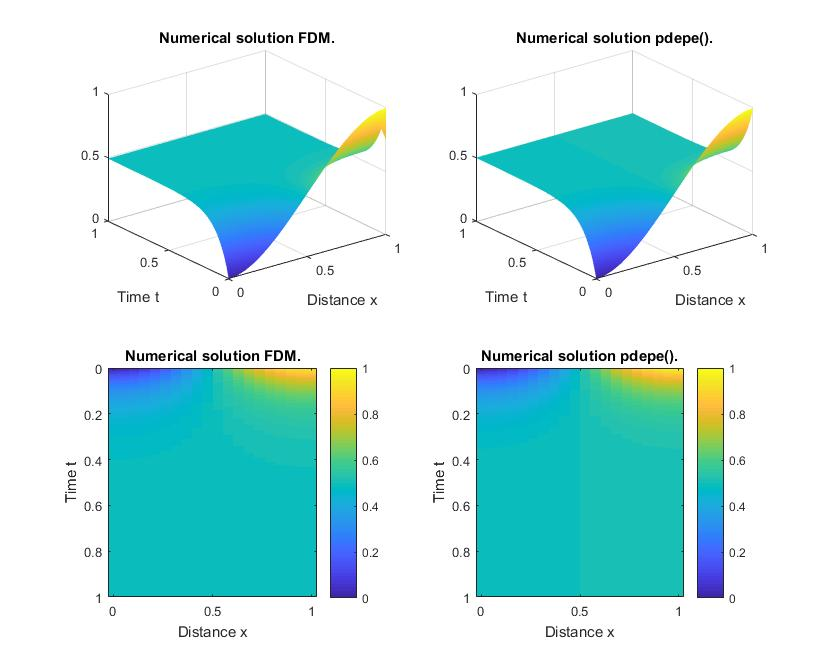
\includegraphics[width=\textwidth,height=\textheight,keepaspectratio]{MATLAB/A1.jpg}
	\end{center}
	\caption{Numerical solutions to case A}
\end{figure}
\begin{figure}
	\begin{center}
		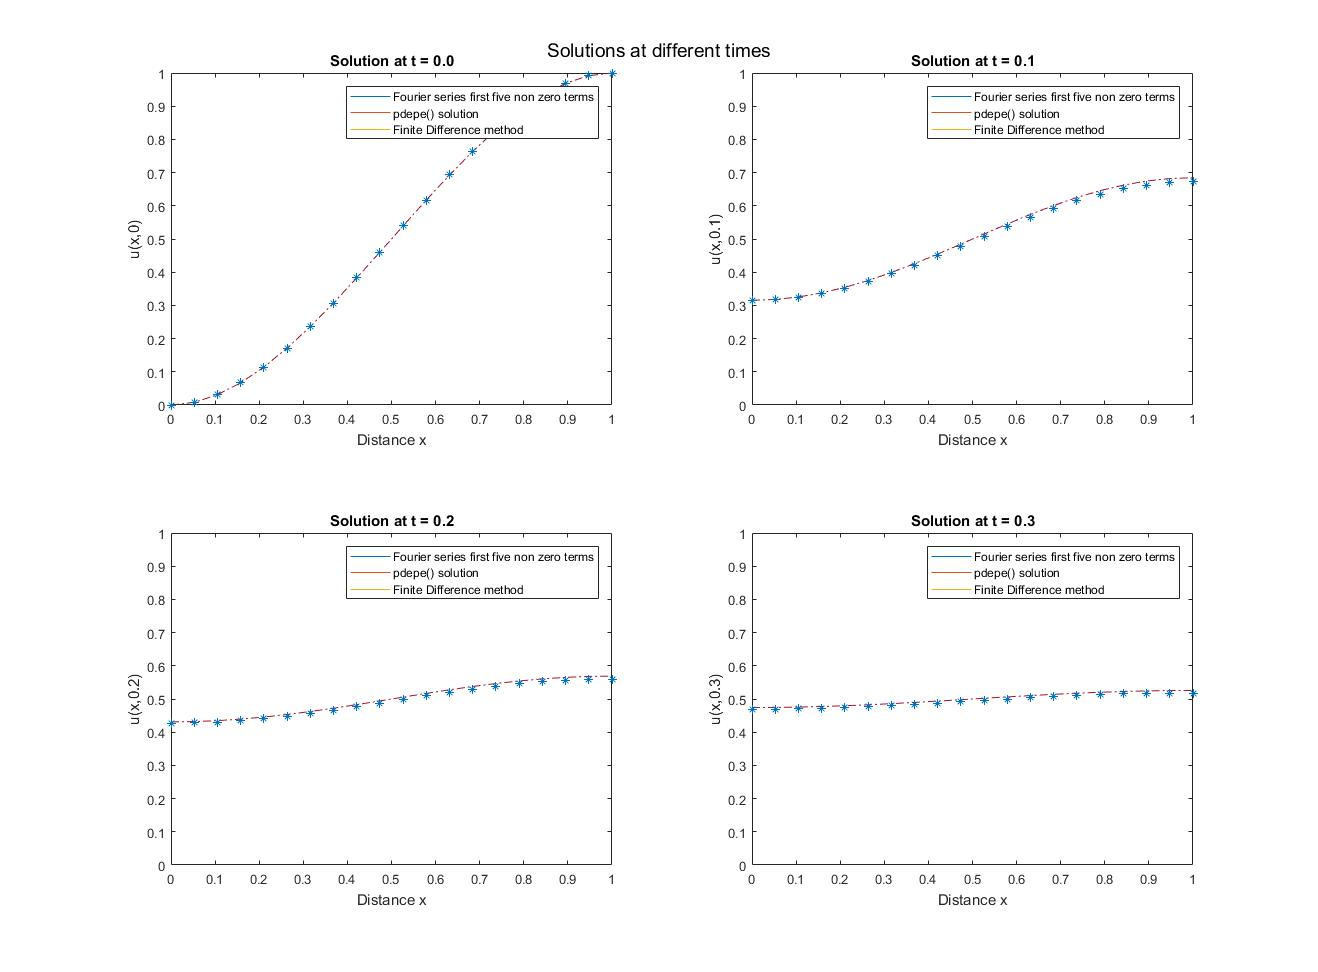
\includegraphics[width=\textwidth,height=\textheight,keepaspectratio]{MATLAB/A2.jpg}
	\end{center}
	\caption{Comparison of the solutions at different t values.}
\end{figure}
\begin{figure}
	\begin{center}
		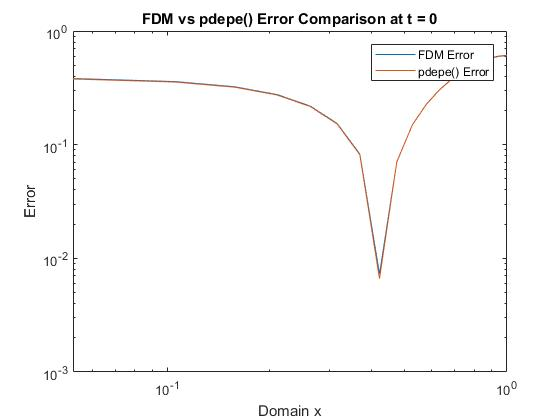
\includegraphics[width=\textwidth,height=\textheight,keepaspectratio]{MATLAB/A3.jpg}
	\end{center}
	\caption{Comparison of error at the initial state}
\end{figure}
%----------------------------------------------------------------------------------------
\newpage
\subsection{Case B: Homogeneous Dirichlet Boundary Condition}
In this example, particles are simply eliminated when the boundaries are reached. Extending the boundaries to a large interval allows us to estimate how particles distribute on a infinite domain, but we utilize the diffusion equation on an infinite domain equation to generate a more accurate model.
\\
\\
\noindent Boundary and initial conditions,
\[
	\begin{split}
		u(0,t) &= 0 \\
		u(1,t) &= 0 \\
		u(x,0) &= x-x^2 \\
	\end{split}
\]
For the Fourier series, we have,
\[
	\begin{split}
		A_n &= 2\int_{0}^{1} (x-x^2)\sin{\left(n\pi x\right)} \ dx \\
		&= 2\left(-\dfrac{{\pi}n\sin\left({\pi}n\right)+2\cos\left({\pi}n\right)-2}{{\pi}^3n^3}\right)
	\end{split}
\]
\[
	\therefore \ u(x,t) = \sum^{\infty}_{n=0} A_n\sin{\left(n\pi x\right)}e^{-kt\left(n\pi\right)^2}
\]
In this case, the density of particles should drop off as time passes.
\\
\\
\noindent DiffEquationZeroBC.m
\begin{lstlisting}[language=Matlab]
% Solutions to the diffusion equation with initial condition x-x^2 and
% zero Dirichlet boundary condition
function DiffEquationZeroBC
clear;
close all;

% Initial variables.
D=1; % Diffusion coefficient.
x_min=0; % Min domain
x_max=1; % Max domain
t_max=1; % Max time
xv=linspace(x_min,x_max,20); % Spatial vector 
dx=xv(2)-xv(1); % x step size
dt=0.5*(dx^2)/(2*D); % t stable step size
tv=0:dt:t_max; % Time vector

% Fourier series solution.
a0=0;
% Series for the domain [0,1]. Requires recalculation should domain change.
series=@(x,t,n)2*(-(pi*n*sin(pi*n)+2*cos(pi*n)-2)/(pi^3*n^3))*sin(n*pi*x)*exp(-(n*pi)^2*t);

% FDM Solution
ic=@(x)x.*(1-x);
fdmU=FDM(1,dx,dt,[x_min x_max],[0 t_max],[0 0],ic);
fdmU=fdmU';

% pdepe Solution
sol=pdepe(0,@pdex1pde,@pdex1ic,@pdex1bc,xv,tv);
% Extract the first solution component as u.
pdepeU=sol(:,:,1);

% Plotting 3D Graphs
figure
subplot(2,2,1)
surf(xv,tv,fdmU)
title('Numerical solution FDM.')
xlabel('Distance x')
ylabel('Time t')
shading interp

subplot(2,2,2)
surf(xv,tv,pdepeU) 
title('Numerical solution PDEPE.')
xlabel('Distance x')
ylabel('Time t')
shading interp

subplot(2,2,3)
imagesc(xv,tv,fdmU) 
title('Numerical solution FDM.')
xlabel('Distance x')
ylabel('Time t')
shading interp
colorbar

subplot(2,2,4)
imagesc(xv,tv,pdepeU) 
title('Numerical solution PDEPE.')
xlabel('Distance x')
ylabel('Time t')
shading interp
colorbar

% Plotting 2D solutions at fixed time t
figure
suptitle('Solutions at different times')
p1=subplot(2,2,1);
plot(xv,seriesSum(series,xv,0,5),'-',xv,pdepeU(1,:),'-.',xv,fdmU(1,:),'*')
title('Solution at t = 0.0')
xlabel('Distance x')
ylabel('u(x,0)')
legend('Fourier series first three non zero terms','pdepe() solution','Finite Difference method')

p2=subplot(2,2,2);
plot(xv,seriesSum(series,xv,0.1,5),xv,pdepeU(round(length(pdepeU)/10)*1,:),'-.',xv,fdmU(round(length(fdmU)/10)*1,:),'*')
title('Solution at t = 0.1')
xlabel('Distance x')
ylabel('u(x,0.1)')
legend('Fourier series first three non zero terms','pdepe() solution','Finite Difference method')

p3=subplot(2,2,3);
plot(xv,seriesSum(series,xv,0.2,5),xv,pdepeU(round(length(pdepeU)/10)*2,:),'-.',xv,fdmU(round(length(fdmU)/10)*2,:),'*')
title('Solution at t = 0.2')
xlabel('Distance x')
ylabel('u(x,0.1)')
legend('Fourier series first three non zero terms','pdepe() solution','Finite Difference method')

p4=subplot(2,2,4);
plot(xv,seriesSum(series,xv,0.3,5),xv,pdepeU(round(length(pdepeU)/10)*3,:),'-.',xv,fdmU(round(length(fdmU)/10)*3,:),'*')
title('Solution at t = 0.3')
xlabel('Distance x')
ylabel('u(x,0.1)')
legend('Fourier series first three non zero terms','pdepe() solution','Finite Difference method')
linkaxes([p1,p2,p3,p4], 'xy');

% Error Figures
figure
loglog(xv,abs((seriesSum(series,xv,0,5))-fdmU(1,:)),xv,abs((seriesSum(series,xv,0,5))-pdepeU(2,:)));
title('FDM vs pdepe() Error Comparison at t = 0')
xlabel('Domain x')
ylabel('Error')
legend('FDM Error', 'pdepe() Error')
xlim([x_min x_max])

% Pdepe function handlers
function [c,f,s]=pdex1pde(x,t,u,DuDx)
c=1;
f=DuDx;
s=0;

function u0=pdex1ic(x)
u0=x*(1-x);

function [pl,ql,pr,qr]=pdex1bc(xl,ul,xr,ur,t)
pl=0;
ql=ul;
pr=0;
qr=ur;
\end{lstlisting}
\begin{figure}
	\begin{center}
		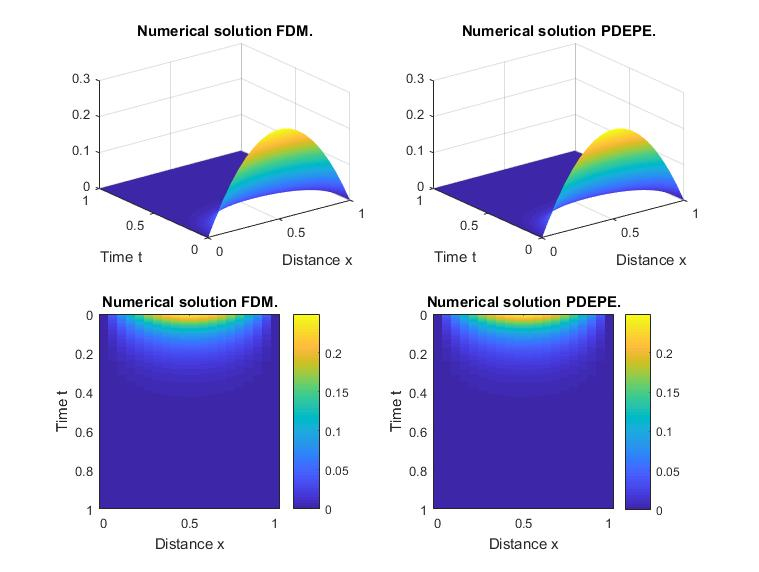
\includegraphics[width=\textwidth,height=\textheight,keepaspectratio]{MATLAB/B1.jpg}
	\end{center}
	\caption{Numerical solutions to case B}
\end{figure}
\begin{figure}
	\begin{center}
		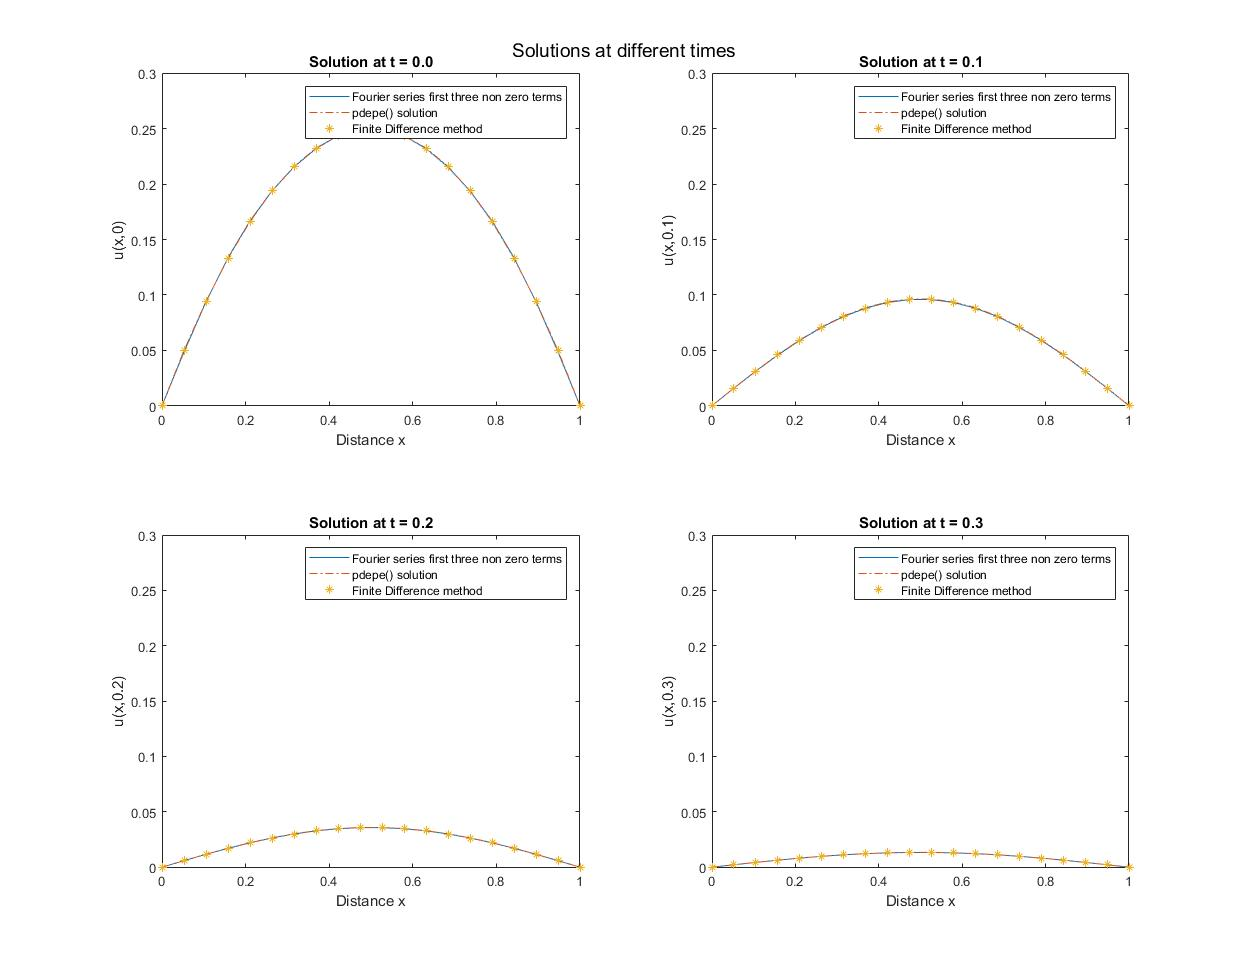
\includegraphics[width=\textwidth,height=\textheight,keepaspectratio]{MATLAB/B2.jpg}
	\end{center}
	\caption{Comparison of the solutions at different t values.}
\end{figure}
\begin{figure}
	\begin{center}
		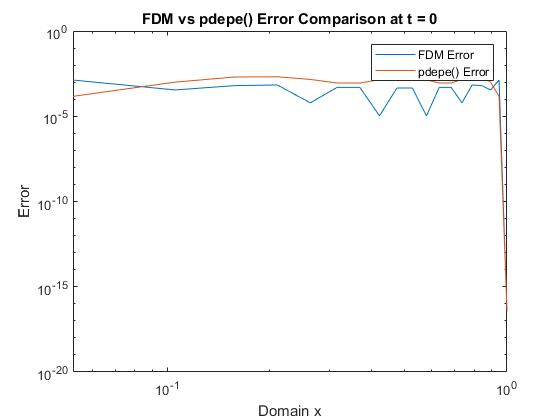
\includegraphics[width=\textwidth,height=\textheight,keepaspectratio]{MATLAB/B3.jpg}
	\end{center}
	\caption{Comparison of error at the initial state}
\end{figure}
%----------------------------------------------------------------------------------------
\newpage
\subsection{Case C: Non-Homogeneous Dirichlet Boundary Condition}
In this example, we will eliminate particles on the left boundary, but have some constant gain on the right.
\\
\\
\noindent Boundary and initial conditions,
\[
	\begin{split}
		u(0,t) &= 0 \\
		u(1,t) &= 1 \\
		u(x,0) &= x^2 \\
	\end{split}
\]
For the Fourier series, we have,
\[
	\begin{split}
		u(x,t) = x + \sum^{\infty}_{n=1} 2\left(\frac{\pi n\sin(\pi n)+2\cos(\pi n)-2}{\pi^3 n^3}\right)\sin(n\pi x)e^{(-(n\pi)^2t)}
	\end{split}
\]
Here we should see that the particles are more denser on the left and begin to drop off towards the right.
\\
\\
\noindent DiffEquationZeroBCNonH.m
\begin{lstlisting}[language=Matlab]
% Solutions to the diffusion equation with initial condition x^2 and
% Non Homogeneous Dirichlet boundary condition
function DiffEquationZeroBCNonH
clear;
close all;

% Initial variables.
D=1; % Diffusion coefficient.
x_min=0; % Min domain
x_max=1; % Max domain
t_max=1; % Max time
xv=linspace(x_min,x_max,20); % Spatial vector 
dx=xv(2)-xv(1); % x step size
dt=0.5*(dx^2)/(2*D); % t stable step size
tv=0:dt:t_max; % Time vector

% Fourier series solution.
a0=xv;
% Series for the domain [0,1]. Requires recalculation should domain change.
series=@(x,t,n)2*((pi*n*sin(pi*n)+2*cos(pi*n)-2)/(pi^3*n^3))*sin(n*pi*x)*exp(-(n*pi)^2*t);

% FDM Solution
ic=@(x)x.^2;
fdmU=FDM(1,dx,dt,[x_min x_max],[0 t_max],[0 1],ic);
fdmU=fdmU';

% pdepe Solution
sol=pdepe(0,@pdex1pde,@pdex1ic,@pdex1bc,xv,tv);
% Extract the first solution component as u.
pdepeU=sol(:,:,1);

% Plotting 3D Graphs
figure
subplot(2,2,1)
surf(xv,tv,fdmU)
title('Numerical solution FDM.')
xlabel('Distance x')
ylabel('Time t')
shading interp

subplot(2,2,2)
surf(xv,tv,pdepeU) 
title('Numerical solution PDEPE.')
xlabel('Distance x')
ylabel('Time t')
shading interp

subplot(2,2,3)
imagesc(xv,tv,fdmU) 
title('Numerical solution FDM.')
xlabel('Distance x')
ylabel('Time t')
shading interp
colorbar

subplot(2,2,4)
imagesc(xv,tv,pdepeU) 
title('Numerical solution PDEPE.')
xlabel('Distance x')
ylabel('Time t')
shading interp
colorbar

% Plotting 2D solutions at fixed time t
figure
suptitle('Solutions at different times')
p1=subplot(2,2,1);
plot(xv,a0+seriesSum(series,xv,0,5),'-',xv,pdepeU(1,:),'-.',xv,fdmU(1,:),'*')
title('Solution at t = 0.0')
xlabel('Distance x')
ylabel('u(x,0)')
legend('Fourier series first three non zero terms','pdepe() solution','Finite Difference method')

p2=subplot(2,2,2);
plot(xv,a0+seriesSum(series,xv,0.1,5),xv,pdepeU(round(length(pdepeU)/10)*1,:),'-.',xv,fdmU(round(length(fdmU)/10)*1,:),'*')
title('Solution at t = 0.1')
xlabel('Distance x')
ylabel('u(x,0.1)')
legend('Fourier series first three non zero terms','pdepe() solution','Finite Difference method')

p3=subplot(2,2,3);
plot(xv,a0+seriesSum(series,xv,0.2,5),xv,pdepeU(round(length(pdepeU)/10)*2,:),'-.',xv,fdmU(round(length(fdmU)/10)*2,:),'*')
title('Solution at t = 0.2')
xlabel('Distance x')
ylabel('u(x,0.1)')
legend('Fourier series first three non zero terms','pdepe() solution','Finite Difference method')

p4=subplot(2,2,4);
plot(xv,a0+seriesSum(series,xv,0.3,5),xv,pdepeU(round(length(pdepeU)/10)*3,:),'-.',xv,fdmU(round(length(fdmU)/10)*3,:),'*')
title('Solution at t = 0.3')
xlabel('Distance x')
ylabel('u(x,0.1)')
legend('Fourier series first three non zero terms','pdepe() solution','Finite Difference method')
linkaxes([p1,p2,p3,p4], 'xy');

% Error Figures
figure
loglog(xv,abs((a0+seriesSum(series,xv,0,5))-fdmU(1,:)),xv,abs((a0+seriesSum(series,xv,0,5))-pdepeU(2,:)));
title('FDM vs pdepe() Error Comparison at t = 0')
xlabel('Domain x')
ylabel('Error')
legend('FDM Error', 'pdepe() Error')
xlim([x_min x_max])

% Pdepe function handlers
function [c,f,s]=pdex1pde(x,t,u,DuDx)
c=1;
f=DuDx;
s=0;

function u0=pdex1ic(x)
u0=x^2;

function [pl,ql,pr,qr]=pdex1bc(xl,ul,xr,ur,t)
pl=0;
ql=ul;
pr=0;
qr=ur-1;
\end{lstlisting}
\begin{figure}
	\begin{center}
		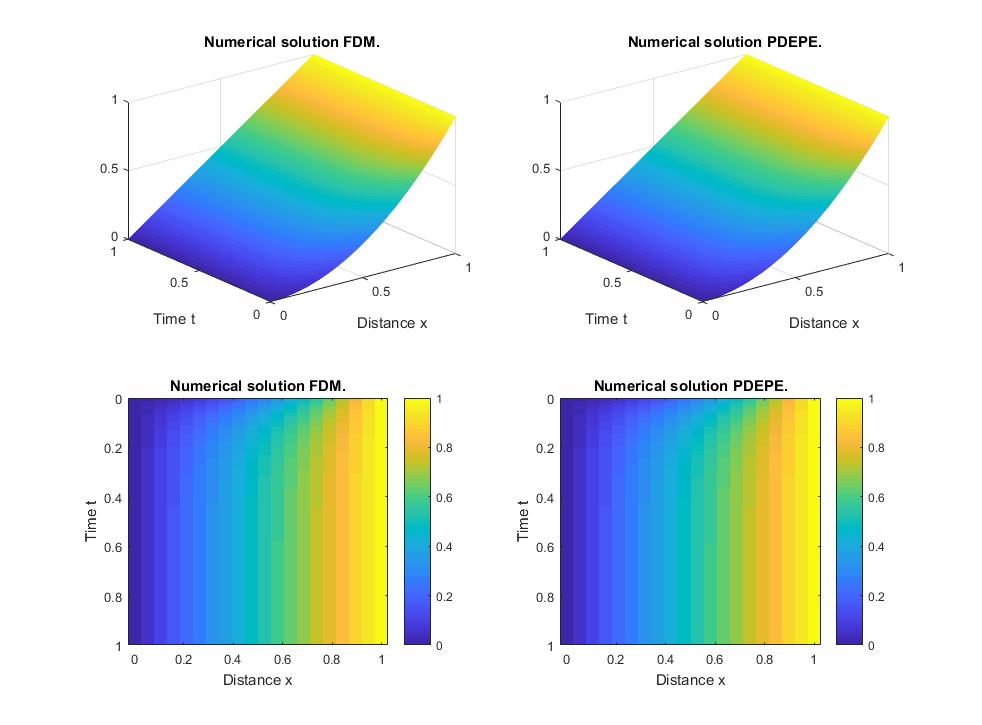
\includegraphics[width=\textwidth,height=\textheight,keepaspectratio]{MATLAB/C1.jpg}
	\end{center}
	\caption{Numerical solutions to case C}
\end{figure}
\begin{figure}
	\begin{center}
		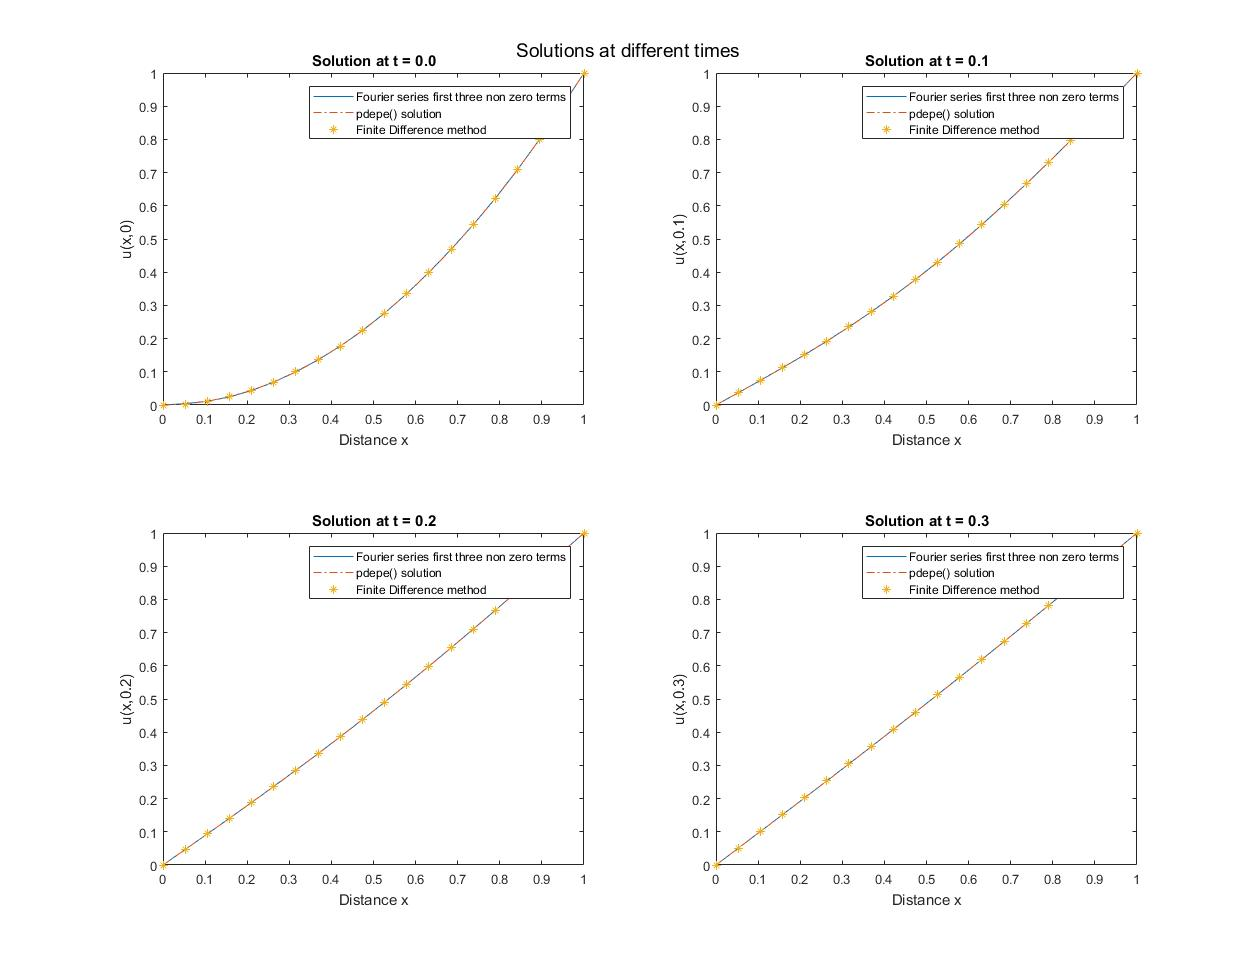
\includegraphics[width=\textwidth,height=\textheight,keepaspectratio]{MATLAB/C2.jpg}
	\end{center}
	\caption{Comparison of the solutions at different t values.}
\end{figure}
\begin{figure}
	\begin{center}
		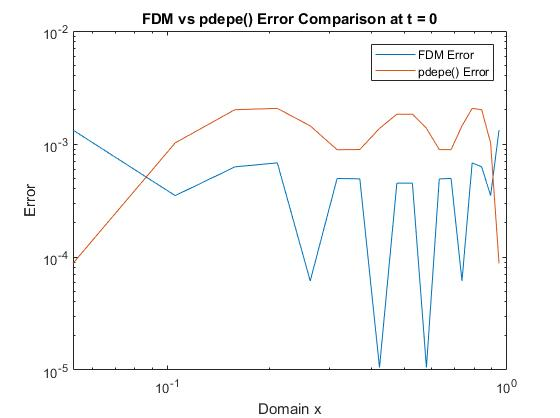
\includegraphics[width=\textwidth,height=\textheight,keepaspectratio]{MATLAB/C3.jpg}
	\end{center}
	\caption{Comparison of error at the initial state}
\end{figure}
\newpage
\subsection{Case D: Non-Linear Model}
\noindent Boundary and initial conditions,
\[
	\begin{split}
		u(0,t) &= 0 \\
		u(1,t) &= 0 \\
	\end{split}
\]
Apply piece-wise steady state solution from section 3.4, we will reach the following formula,
\[ 
	u_s(x) = \begin{cases} 
      0.1x & 0 \leq x < 0.4 \\
      \frac{-x^2}{2} + \frac{1}{2}x - 0.08 & 0.4 \leq x\leq 0.6 \\
      -0.1x + 0.1 & 0.4 < x \leq 1
   \end{cases}
\]
Here a constant area distributing particles is placed in the middle, we should see it distribute over the surface area over time.
\begin{lstlisting}[language=Matlab]
function DiffusionEquationNonLinear

clear;
close all;

% Setup constants and vectors.
D=1;
dx=0.02;
x_vec=0:dx:1;
dt=0.5*(dx^2)/(2*D);
t_vec=0:dt:1;

% Solve the system with FDM
U=FDMInitial(D,dx,dt,[0 1],[0 1],[0 0],0,[0.4 0.6]);
U=U';

% 3D Plot of the numerical solution.
figure
surf(x_vec,t_vec,U);
title('Numerical Solution');
xlabel('Space');
ylabel('Time');
shading interp
colorbar

% Plot the numerical solution.
figure
imagesc(t_vec,x_vec,U);
colorbar;
title('Numerical Solution');
xlabel('Space');
ylabel('Time');

% Plot the defined steady state solution.
figure
hold on
x1 = 0:0.01:0.4;
x2 = 0.4:0.01:0.6;
x3 = 0.6:0.01:1;
y1 = 0.1*x1;
y2 = -(x2.^2/2)+0.5.*x2-0.08;
y3 = -0.1.*x3+0.1;
plot(x_vec,U(end,:),x1,y1,'r',x2,y2,'r',x3,y3,'r');
title('Solution at t = 1');
xlabel('x');
ylabel('U(x)');
legend('Numerical Solution', 'Exact')
\end{lstlisting}
\begin{figure}[bp!]
	\begin{center}
		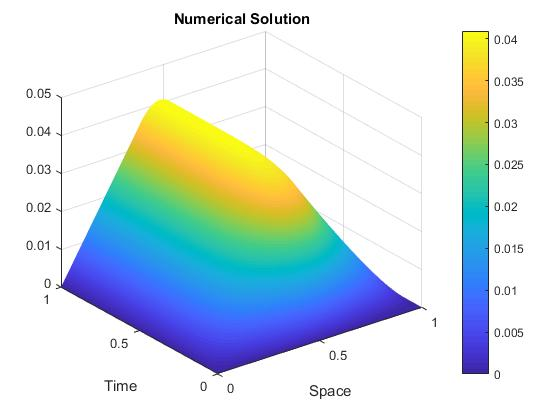
\includegraphics[width=\textwidth,height=\textheight,keepaspectratio]{MATLAB/D1.jpg}
	\end{center}
	\caption{Numerical solutions to case A}
\end{figure}
\begin{figure}
	\begin{center}
		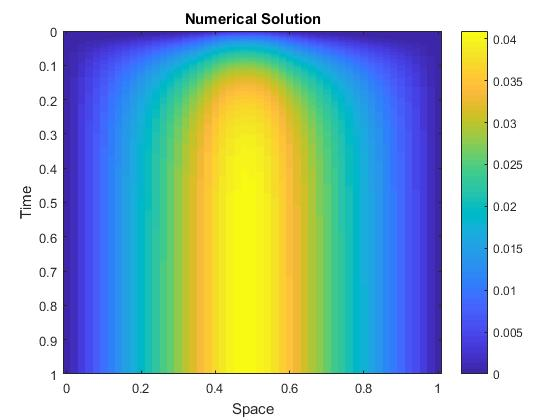
\includegraphics[width=\textwidth,height=\textheight,keepaspectratio]{MATLAB/D2.jpg}
	\end{center}
	\caption{Comparison of the solutions at different t values.}
\end{figure}
\begin{figure}
	\begin{center}
		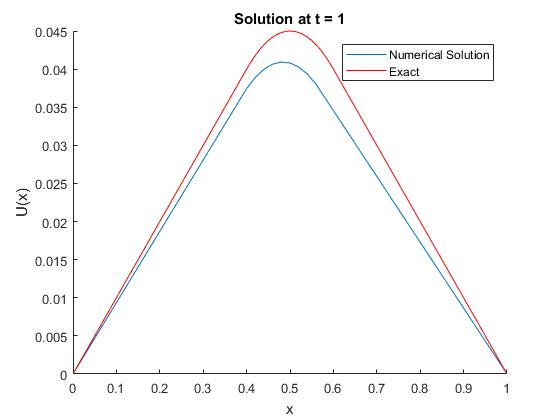
\includegraphics[width=\textwidth,height=\textheight,keepaspectratio]{MATLAB/D3.jpg}
	\end{center}
	\caption{Comparison of the solution at t = 1 (Steady state solution)}
\end{figure}
\newpage
We can improve this numerical solution by reducing the step size. However, due to our restriction of the step sizes for $x$ and $t$, the memory required for the matrix will grow a size too great for an average computer to handle. Take $\triangle x = 0.001$ then $\triangle t = 0.00000025$ results in a 1000 by 4000000 array of 4000000000 elements and according to MATLAB will require approximately 30GB.
\\
\\
Below we have a few more examples of this type. Simply modify the bounds within FDMInitial.m to achieve these results.
\begin{figure}
	\begin{center}
		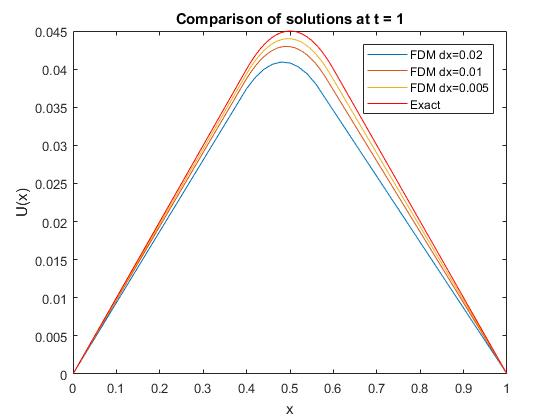
\includegraphics[width=\textwidth,height=\textheight,keepaspectratio]{MATLAB/D4.jpg}
	\end{center}
	\caption{Comparison of the solution at t = 1 (Steady state solution)}
\end{figure}
\begin{figure}
	\begin{center}
		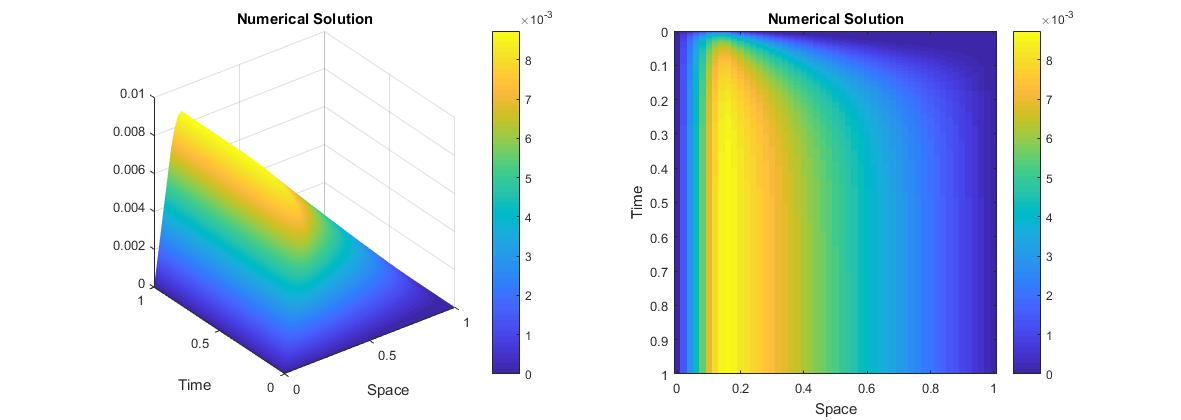
\includegraphics[width=\textwidth,height=\textheight,keepaspectratio]{MATLAB/D5.jpg}
	\end{center}
	\caption{Diffusion field at 0.1 to 0.2}
\end{figure}
\begin{figure}
	\begin{center}
		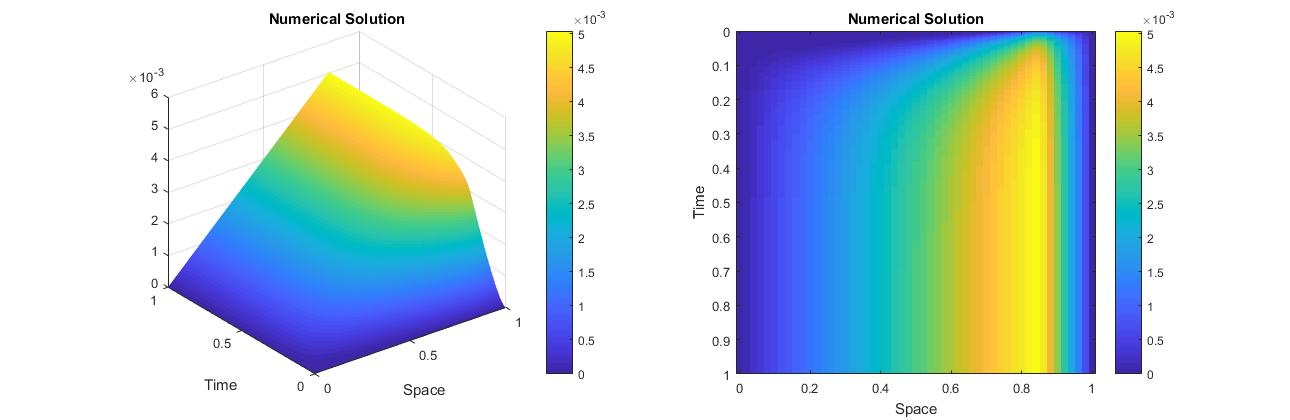
\includegraphics[width=\textwidth,height=\textheight,keepaspectratio]{MATLAB/D6.jpg}
	\end{center}
	\caption{Diffusion field at 0.8 to 0.9}
\end{figure}
\begin{figure}
	\begin{center}
		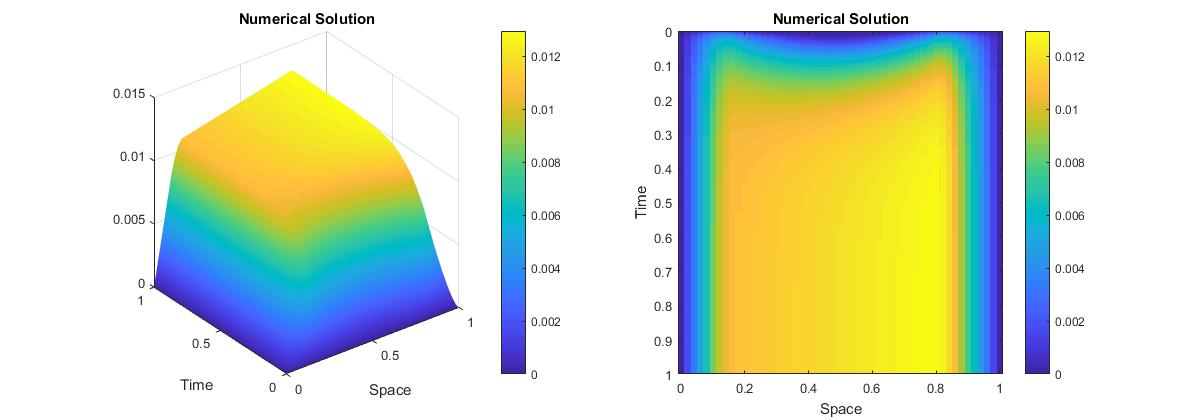
\includegraphics[width=\textwidth,height=\textheight,keepaspectratio]{MATLAB/D7.jpg}
	\end{center}
	\caption{Diffusion field at 0.1 to 0.2 and 0.8 to 0.9}
\end{figure}
\newpage
\section{Discussion}
\subsection{Accuracy \& Error}
From the cases we tested, it is clear that pdepe() and the Finite Difference Scheme are both effective for solving the diffusion equation. Both methods generated solutions of reasonable accuracy with the Finite Difference Scheme being slightly more accurate than pdepe(). In the error comparison graphs, the error takes a sinusoidal form indicating the truncation error formed from the Fourier series.
\\
\\
In the first case, where we defined a system with Homogeneous Dirichlet Boundary Condition we can see that the particle density over the area simply flattens out and distributes evenly, thus following our estimations. Errors from both methods are about the same with the Finite Difference Method just a small advantage in terms of accuracy. In the second case the system is defined to lose particles which reach the boundary resulting in the system to decrease in density of particles adhering to our estimations. The third case represents a system with a out-flux on the left and a influx on the left, as we lose particles in the system, we also gain them. According to the graphs, the density is much greater on the influx side and approaches zero on the out-flux side. Here the distinction in error is much clearer, with pdepe() the errors are consistently higher than FDM, with the exception of the initial points. FDM on the other hand has unstable spikes of different error, although the amplitude of the error oscillation is lower than the pdepe() approximation. Finally, in the last case, we utilized a different type of diffusion equation with an additional term defined as non zero for only a certain region. This region will apply a constant particle distribution across the area but is eliminated when the boundaries are reached, hence we see a triangle like graph of particles diffusing. Here we did not apply the pdepe solution since we only tested the steady state solution, and instead considered only the Finite Difference Scheme.
\begin{figure}[hp]
	\begin{center}
		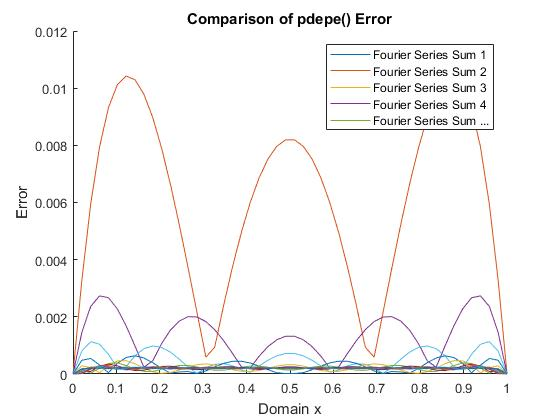
\includegraphics[width=\textwidth,height=\textheight,keepaspectratio]{MATLAB/Err1.jpg}
	\end{center}
	\caption{pdepe() Error reduces and approaches 0 as terms increase in the Fourier Series (ErrorComparison.m)}
\end{figure}
\newpage
\begin{figure}[hp]
	\begin{center}
		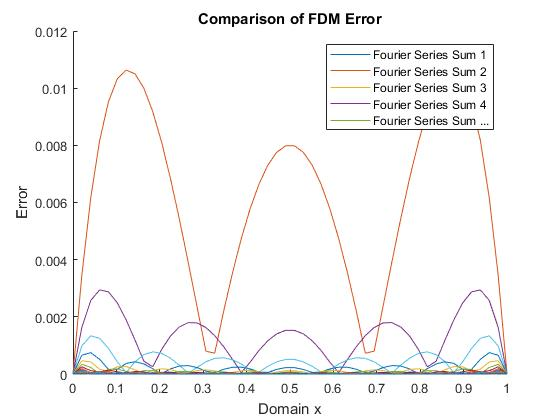
\includegraphics[width=\textwidth,height=\textheight,keepaspectratio]{MATLAB/Err2.jpg}
	\end{center}
	\caption{FDM Error reduces and approaches 0 as terms increase in the Fourier Series (ErrorComparison.m)}
\end{figure}

\noindent While the FDM appears to be more accurate, the size of the matrix exponentially grows as the step size is reduced. Additionally, the step size are bounded by a condition, should it not be satisfied, the solution will become unstable and thus outputting an invalid solution.
\\
\\
Truncation error of the Fourier Series will be of an concern if not enough correct terms are used, additionally, the operators and approximation to compute exponential, sines or cosine functions also contribute to the round off error of the final approximation. In our test cases, we chose to sum up to the first five non zero terms, although higher values could be used, the five terms was "good enough" for our comparisons.
\newpage
\subsection{Time Complexity}
The runtime of both methods greatly differ, with pdepe() taking significantly longer to compute solutions of the same grid points. Both methods show no signs or patterns of growing runtimes but this could be due to the max grid points we chose to compute which was 100. Setting this to a higher value would first increase memory usage to store the matrices and second, prolong our script to generate these runtimes.
\begin{figure}[hp]
	\begin{center}
		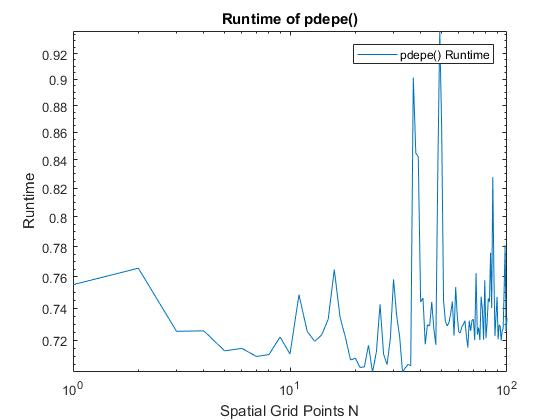
\includegraphics[width=\textwidth,height=\textheight,keepaspectratio]{MATLAB/pdepeRuntime.jpg}
	\end{center}
	\caption{Runtime of pdepe() as grid points increased (Runtime.m)}
\end{figure}
\newpage
\begin{figure}[hp]
	\begin{center}
		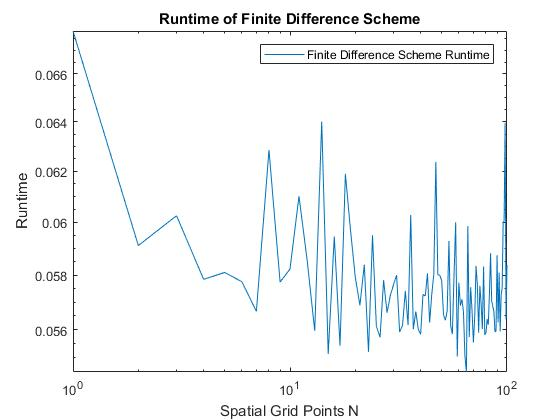
\includegraphics[width=\textwidth,height=\textheight,keepaspectratio]{MATLAB/FDMRuntime.jpg}
	\end{center}
	\caption{Runtime of pdepe() as grid points increased (Runtime.m)}
\end{figure}
A potential reason for the longer runtime of pdepe() could be due to the way the method was implemented. pdepe() takes function handles to define its initial state and within the function itself, checks for arguments, event handlers and other verification methods, all of which requires service routines to be called thus prolonging the script execution time. We can estimate that stiff system was not a cause since the solution in our domain showed no qualities of a stiff system and pdepe() relies on ode15s(), a low order method to compute its time integrals.
\newpage
\begin{figure}[hp]
	\begin{center}
		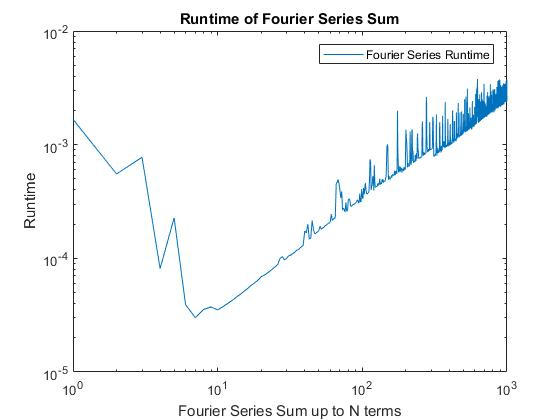
\includegraphics[width=\textwidth,height=\textheight,keepaspectratio]{MATLAB/FSRuntime.jpg}
	\end{center}
	\caption{Runtime of Summation of the Fourier Series as the terms to sum up to increased (Runtime.m)}
\end{figure}
Additionally, we tested the Fourier series summation runtimes, however this is a trivial result since summation methods generally has a time complexity of O($n$) and as verified by the graph above, does indeed follow that pattern. The initial high values and spikes seen throughout the plots are usually due to the system handling other services and applications.
\newpage
\subsection{Problems Encountered}
Throughout creating the scripts for the cases, one problem major I encountered was the lack of documentation of the pdepe() function, especially in setting the boundary condition. The function handler, handling the boundary condition utilizes variable with no comments thus leading to cases where attempting to set zero boundary conditions or influx of particles did not match the Fourier Series solution despite the setup of the boundary condition "looking correct".
\section{Conclusion}
In conclusion, this research provided deep insights into the workings of the Finite Difference Scheme and pdepe(). We created different variations of the methods and utilized it to solve different cases of the diffusion, of which every single case matched our estimation and the analytical solution. The Finite Difference Scheme was much more accurate but is constrained by the step size chosen for the time and spatial domains and may result in large memory required to compute more complex systems. Although our models were simple, deriving the analytical solutions for verification will become much more difficult should the model be slightly more complex. These models are very interesting to compute, especially the slightly more complex cases, should I attempt this again, I would focus on one specific case, but increase the complexity of the models for a more realistic simulation.
%----------------------------------------------------------------------------------------
\end{document}
